\chapter{Curvas Caracteristicas}
  El comportamiento eléctrico del transistor BJT puede representarse mediante sus \textbf{curvas características}, que
  describen las relaciones entre corrientes y tensiones en sus terminales bajo diferentes condiciones de polarización.
  Estas curvas permiten identificar claramente las \textit{regiones de operación} del transistor: corte, activa y
  saturación.
    
  Una de las curvas más representativas es la familia de curvas $I_C$ vs.\ $V_{CE}$ para distintos valores de $I_B$.
  Estas muestran cómo varía la corriente de colector en función de la tensión colector-emisor, manteniendo constante la
  corriente de base. Esta representación permite visualizar:
    
  \begin{itemize}
      \item La \textbf{región de corte}: cuando $I_B = 0$, no hay conducción.
      \item La \textbf{región activa}: donde se cumple que $I_C \approx \beta \cdot I_B$.
      \item La \textbf{región de saturación}: donde $V_{CE}$ es bajo y $I_C$ deja de aumentar significativamente.
  \end{itemize}
  
  El análisis experimental de estas curvas, junto con su comparación con resultados simulados y teóricos, permite
  comprender en profundidad el funcionamiento del transistor y validar su modelo de comportamiento.

  \section{Simulacion}
    En esta parte se simula el comportamiento del transistor barrando $V_{CE}$ para distintos valores de $I_B$,
    obteniendo las curvas $I_C$ vs.\ $V_{CE}$. Estas curvas permitieron visualizar claramente las regiones de operación
    del BJT y validar el modelo teórico mediante comparación con los resultados experimentales.

    \begin{figure}[!ht]
      \centering
      \begin{minipage}{0.45\textwidth}
        \begin{tikzpicture}[circuitikz, straight voltages]
          % Paths, nodes and wires:
          \draw node[npn] (N1) at (8, 6.23) {} node[anchor=west] at (N1.text){$BC547B$};
          \draw (7.16, 6.23) to[american resistor, l={$100K \, \Omega$}, label distance=0.02cm] (5, 6.23);
          \draw (8.5, 7.75) to[american resistor, l={$560 \, \Omega$}, label distance=0.02cm] (10.5, 7.75);
          \draw (8, 7) -| (8, 7.75);
          \draw (11, 6.75) to[battery, l={$V_{CC}$}, label distance=0.02cm] (11, 5.75);
          \draw (11, 6.75) -| (11, 7.75);
          \draw (8, 5.46) -- (8, 4);
          \draw (11, 5.75) -- (11, 4);
          \draw node[ground] at (8, 4) {};
          \draw node[ground] at (11, 4) {};
          \draw (8, 7.75) -- (8.5, 7.75);
          \draw (10.5, 7.75) -- (11, 7.75);
          \draw (5, 5.5) to[battery, l={$V_{BB}$}, label distance=0.02cm] (5, 4.5);
          \draw (5, 5.5) |- (5, 6.23);
          \draw (5, 4.5) -| (5, 4);
          \draw node[ground] at (5, 4) {};
        \end{tikzpicture}
        \caption{Circuito de prueba para polarizacion.}
        \label{crkt:curv}
      \end{minipage}
      \hfill
      \begin{minipage}{0.45\textwidth}
        \begin{lstlisting}[style=ltspice, caption={Parámetros de simulación LTspice}, label=list:curv]
.dc VCC 0 10 100m
.step param VBB 0 5 200m
        \end{lstlisting}
      \end{minipage}
    \end{figure}

    \begin{figure}[!ht]
      \centering
      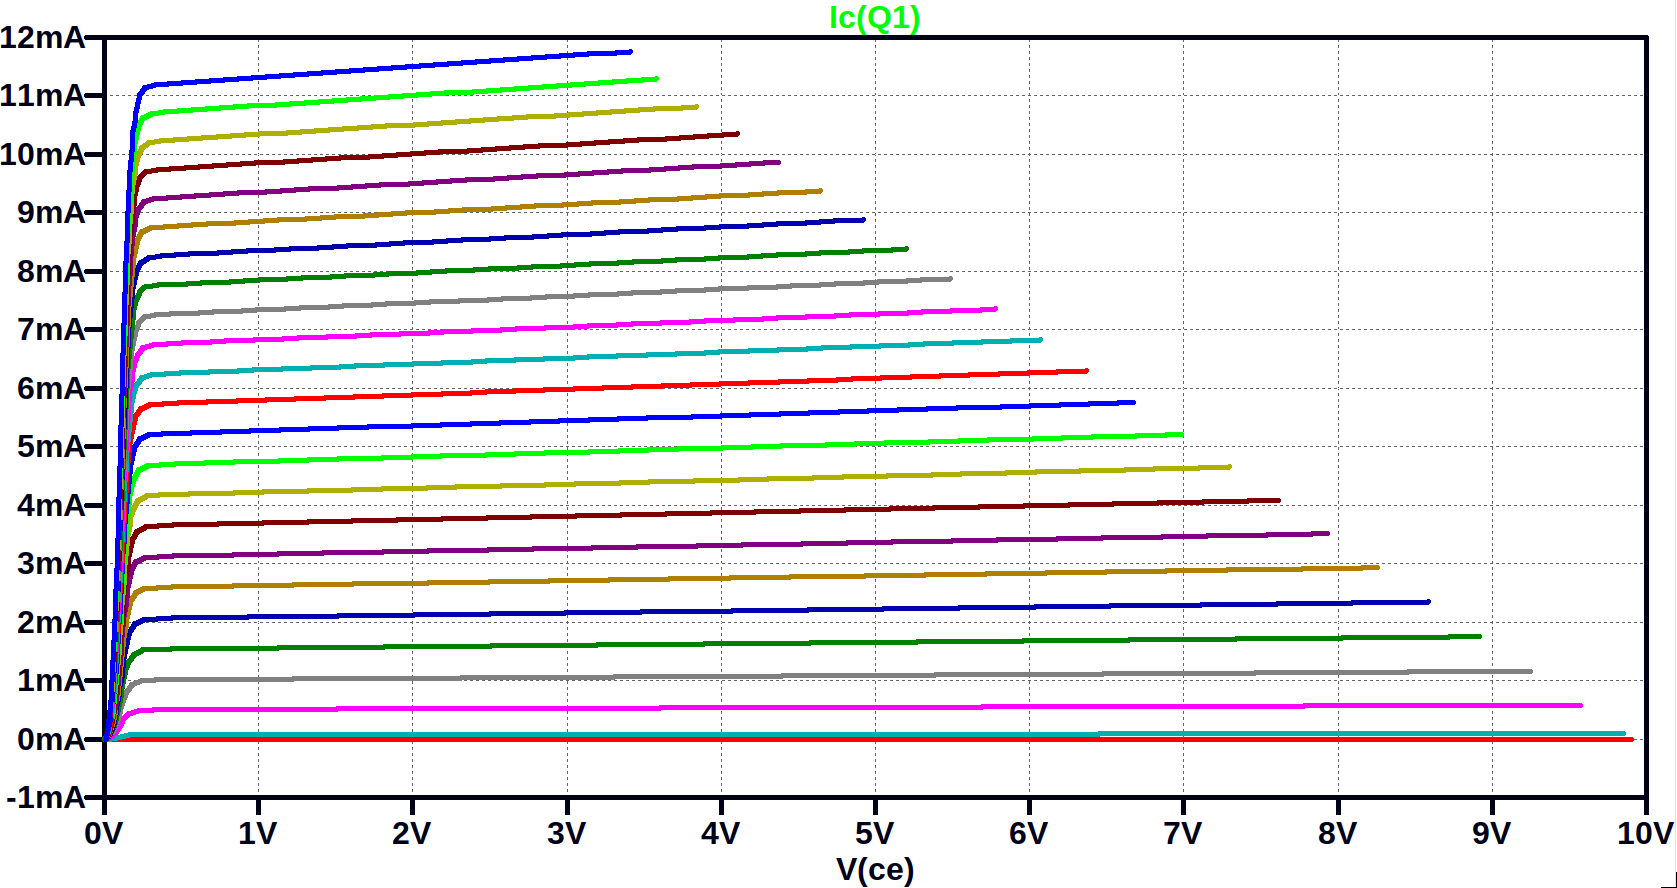
\includegraphics[width=1\textwidth]{images/graph_vce-ic.png}
      \caption{Grafico de corriente del colector respecto a la tension colector-emisor.}
    \end{figure}

  \section{Laboratorio}
    En esta parte se realizaron mediciones experimentales de la corriente de colector $I_C$ en función de la tensión
    colector-emisor $V_{CE}$, para distintos valores de corriente de base $I_B$. Esto permitió identificar las regiones
    de corte, activa y saturación del transistor.

    \begin{figure}[!ht]
      \centering
      \begin{minipage}{0.49\textwidth}
        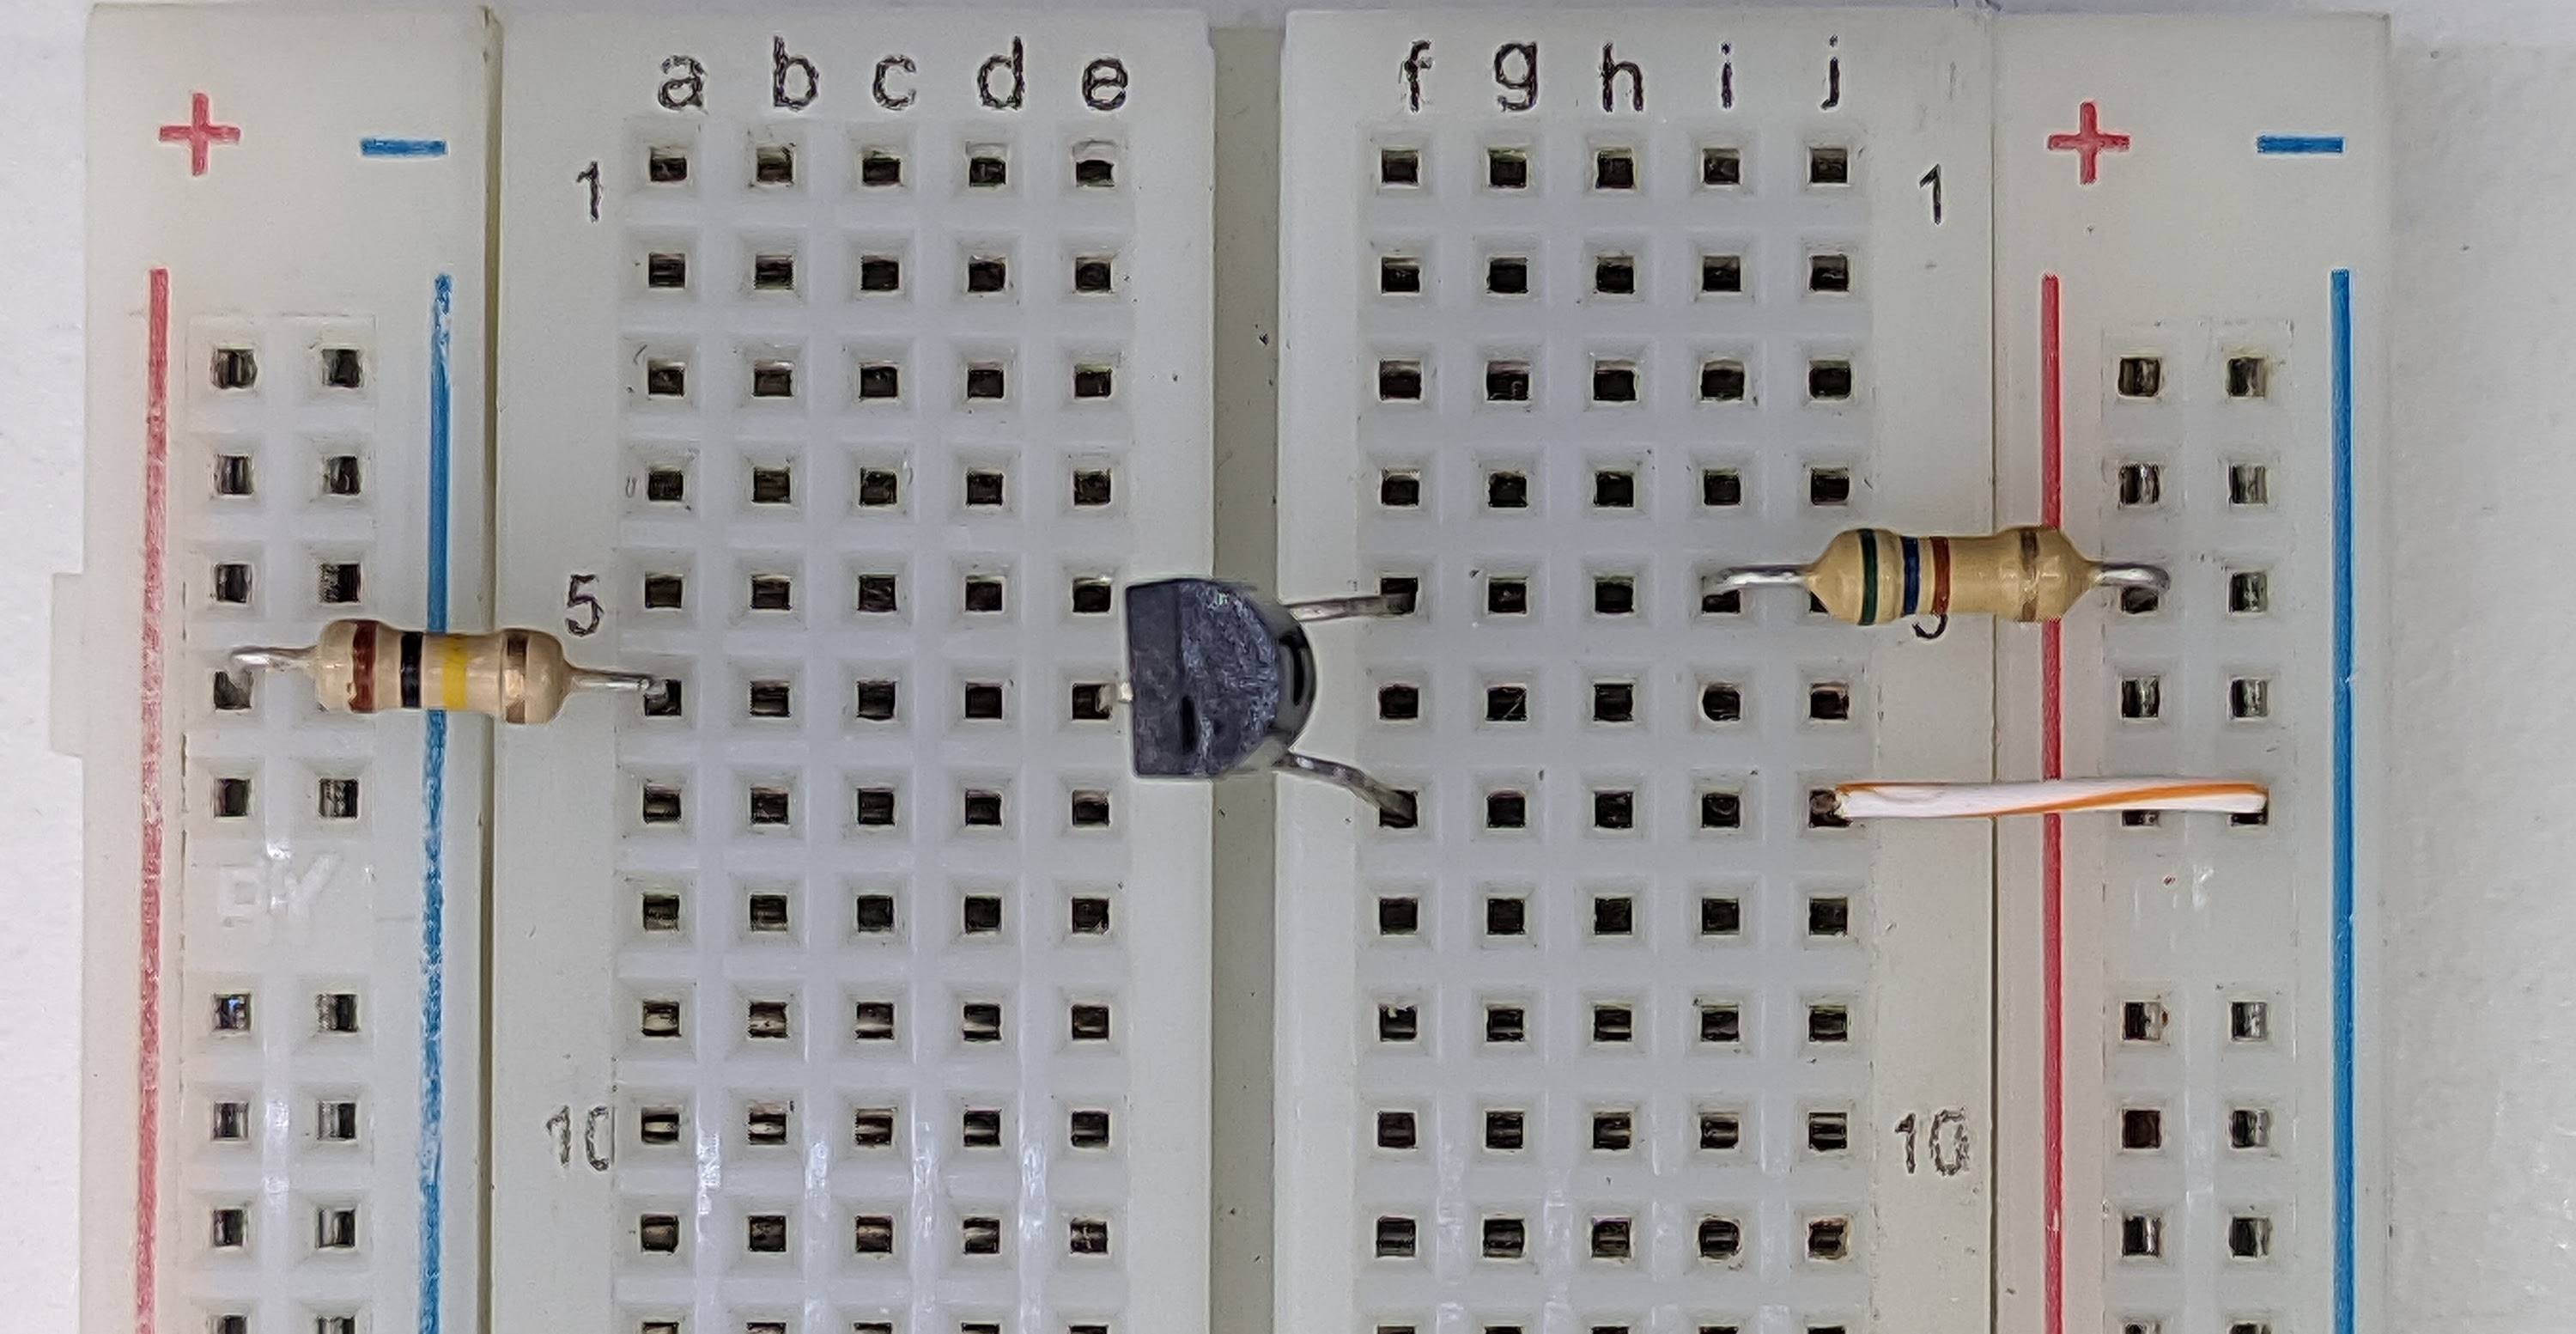
\includegraphics[width=1\textwidth]{pictures/prot_crkt-2_3.jpg}
        \caption{Circuito implementado.}
      \end{minipage}
      \begin{minipage}{0.49\textwidth}
        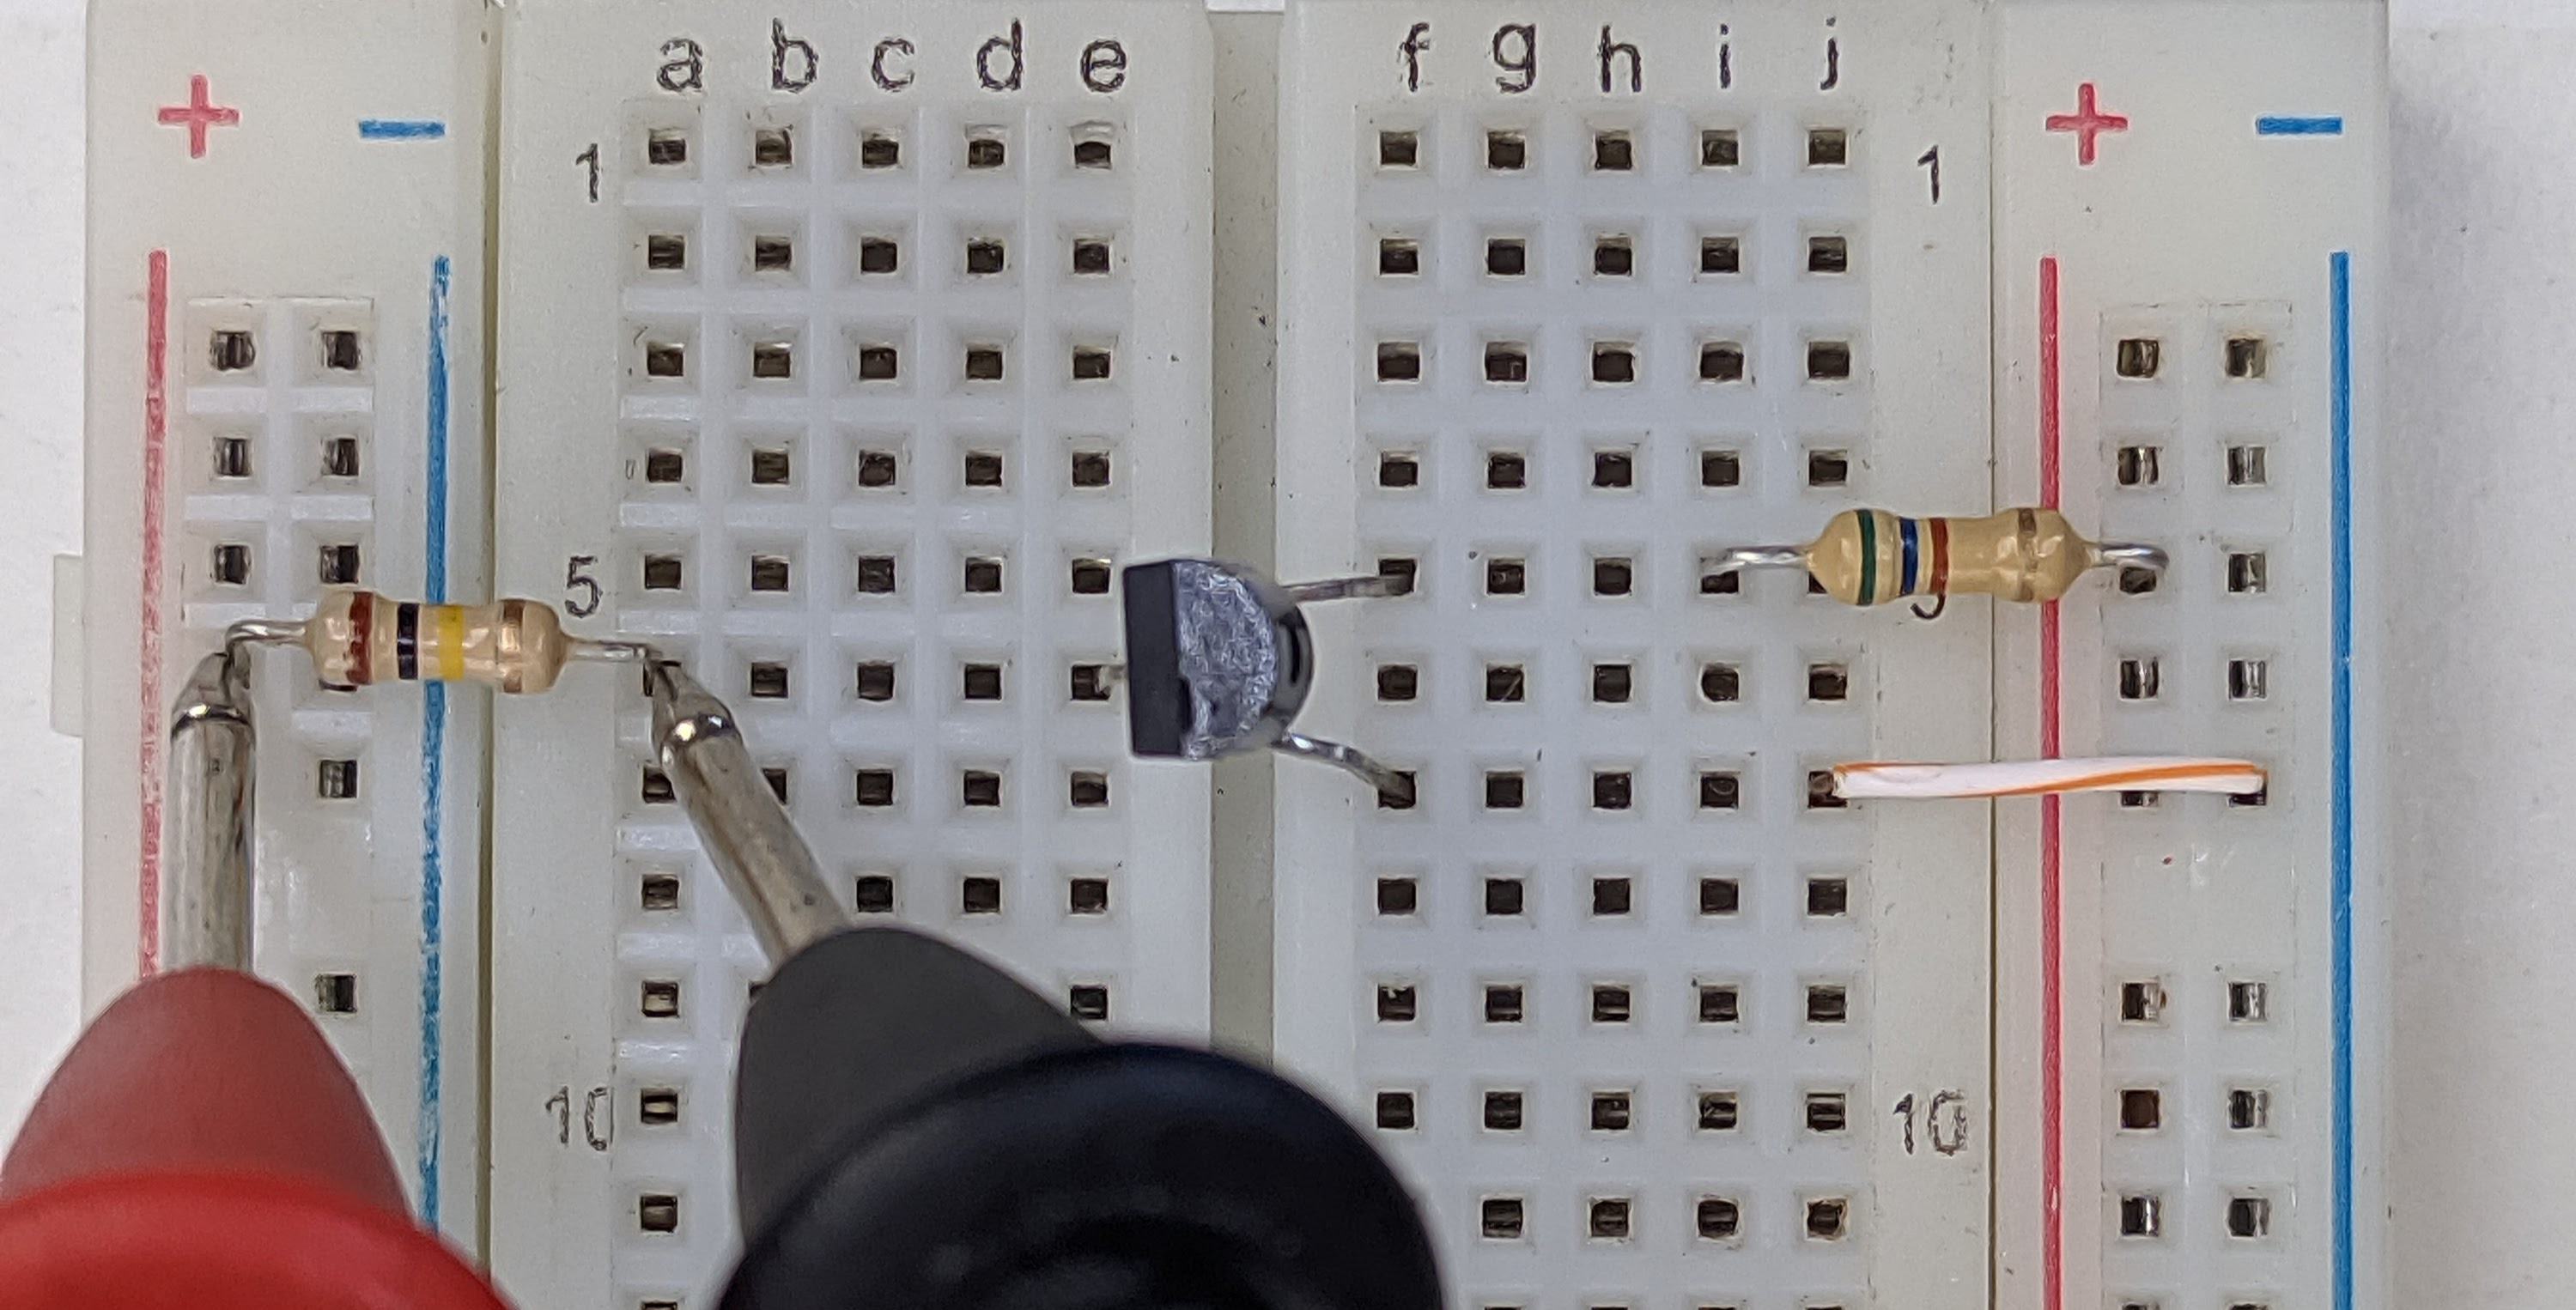
\includegraphics[width=1\textwidth]{pictures/prot_crkt-2_3_Vrb.jpg}
        \caption{Mediciones de $V_{R_B}$.}
      \end{minipage}
    \end{figure}
    \begin{figure}[!ht]
      \centering
      \begin{minipage}{0.49\textwidth}
        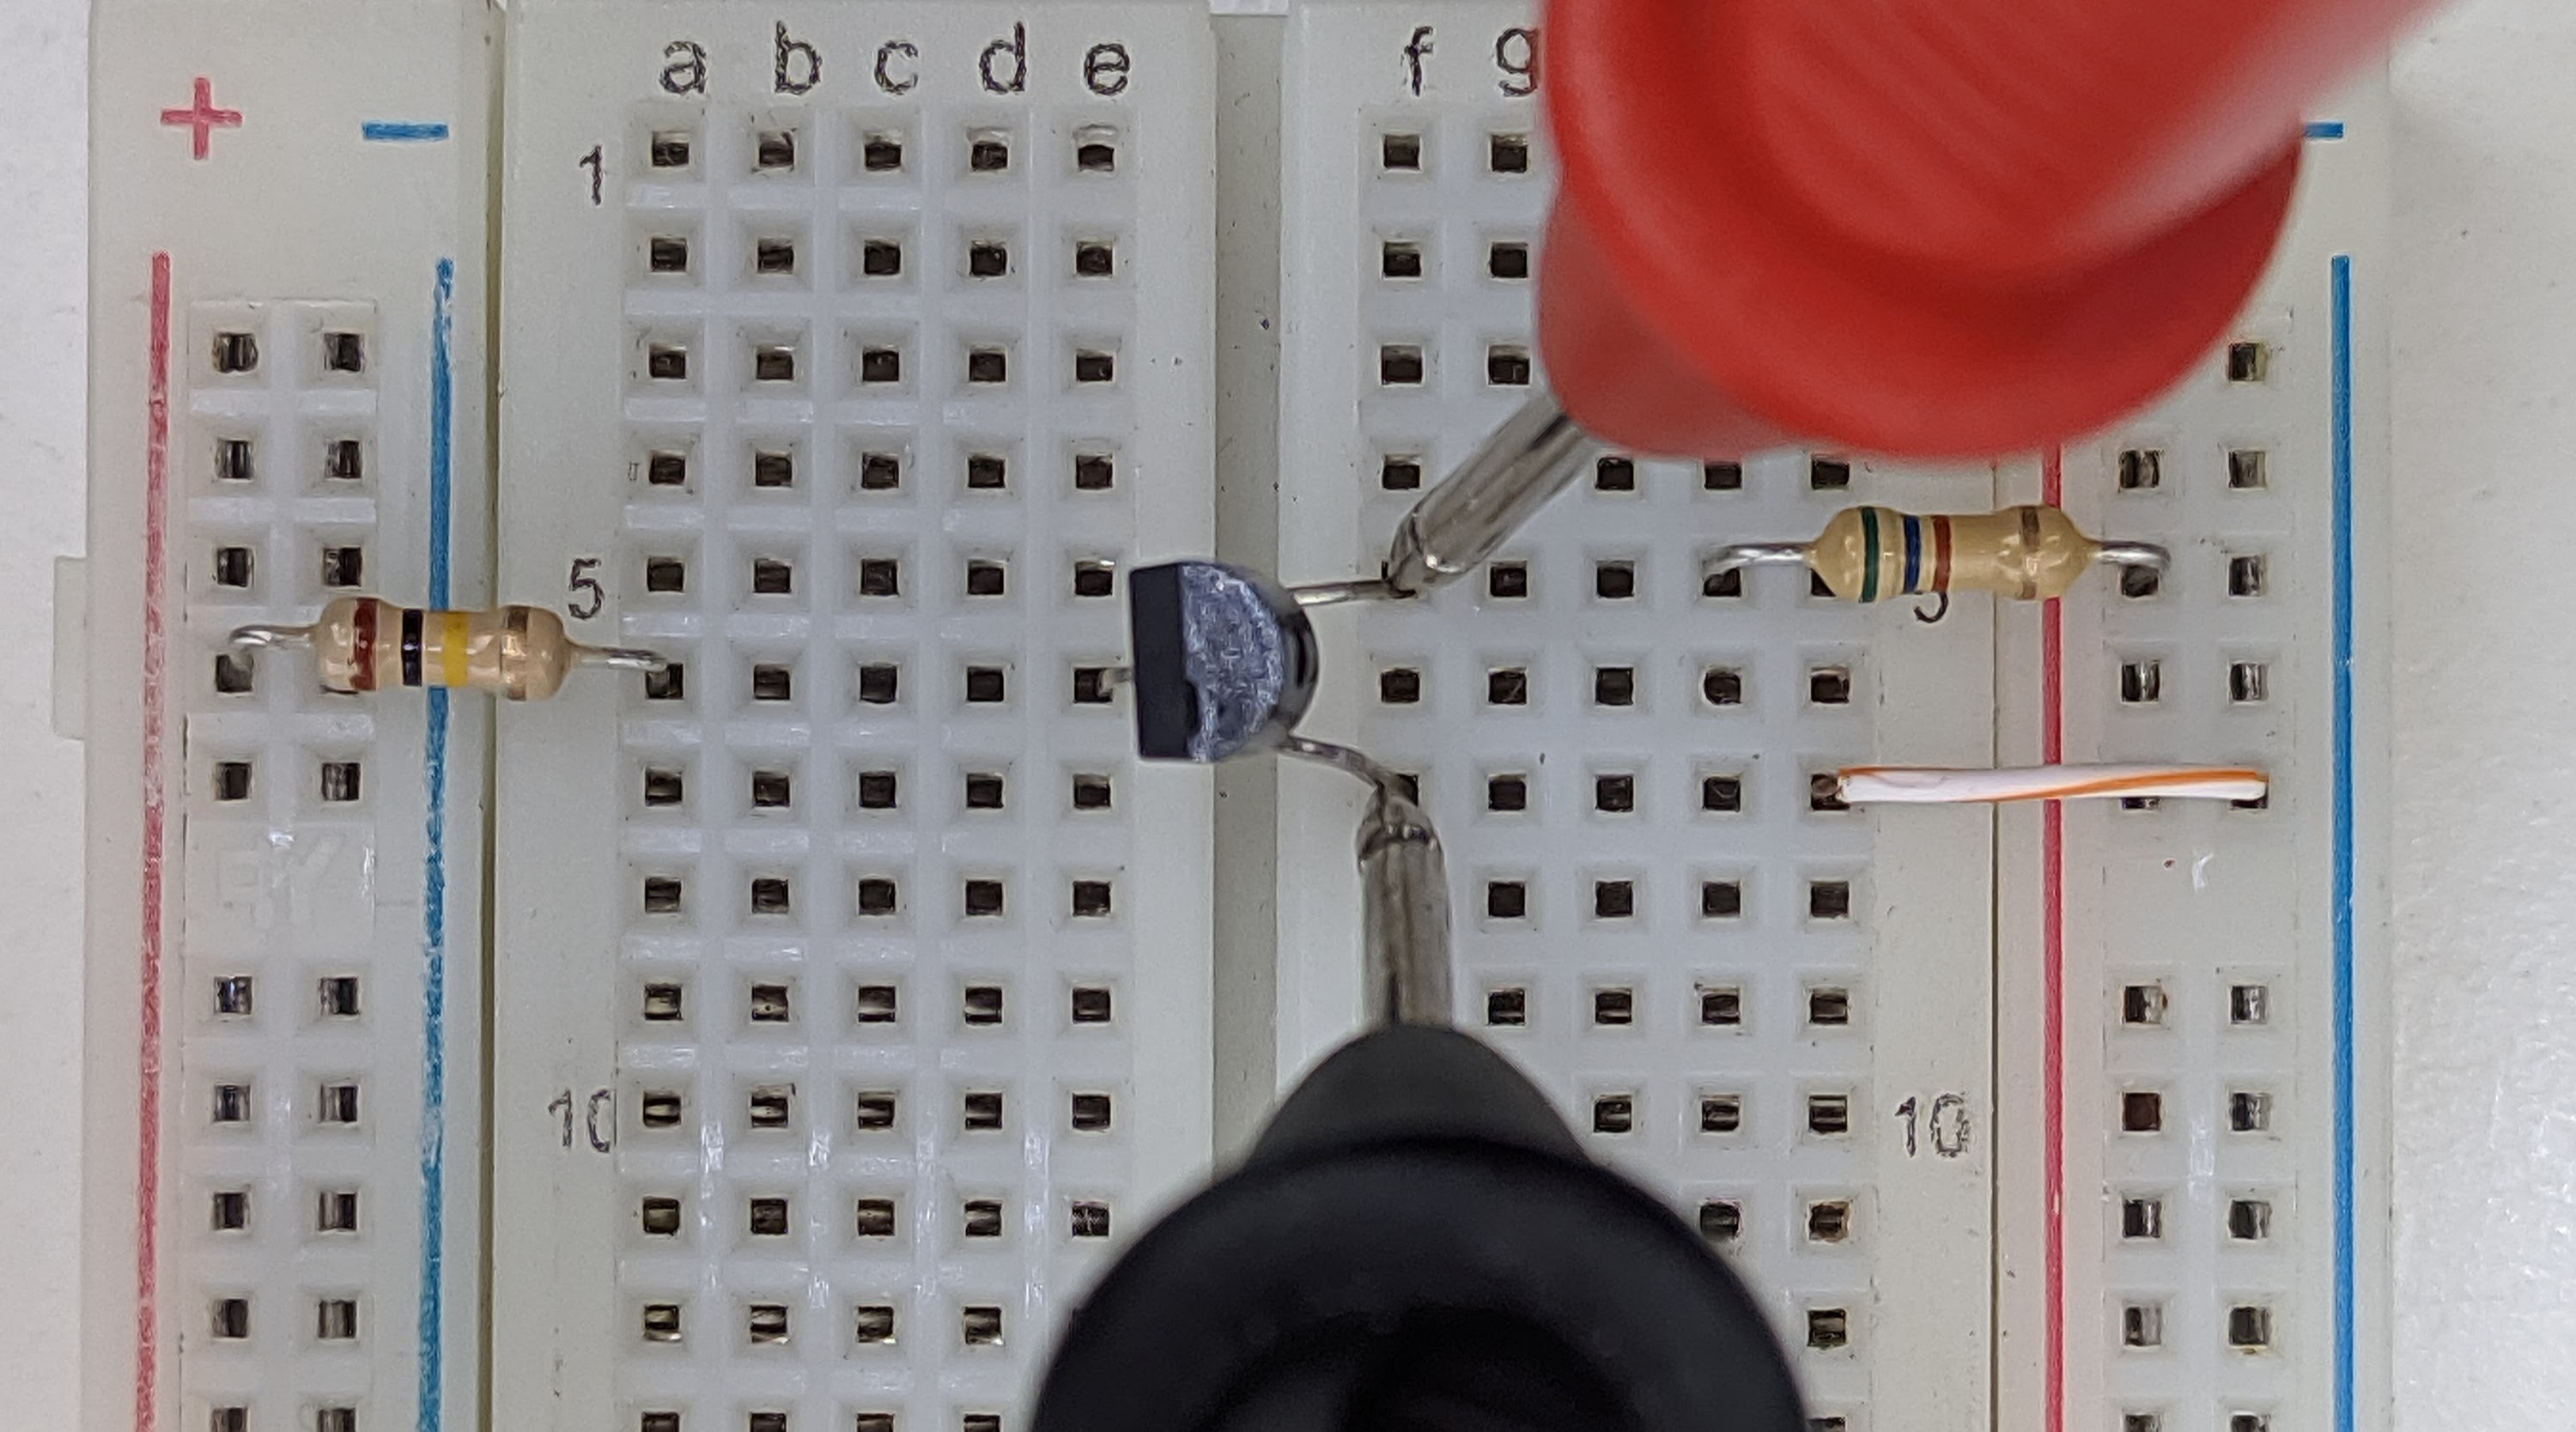
\includegraphics[width=1\textwidth]{pictures/prot_crkt-3_Vce.jpg}
        \caption{Mediciones de $V_{CE}$.}
      \end{minipage}
      \begin{minipage}{0.49\textwidth}
        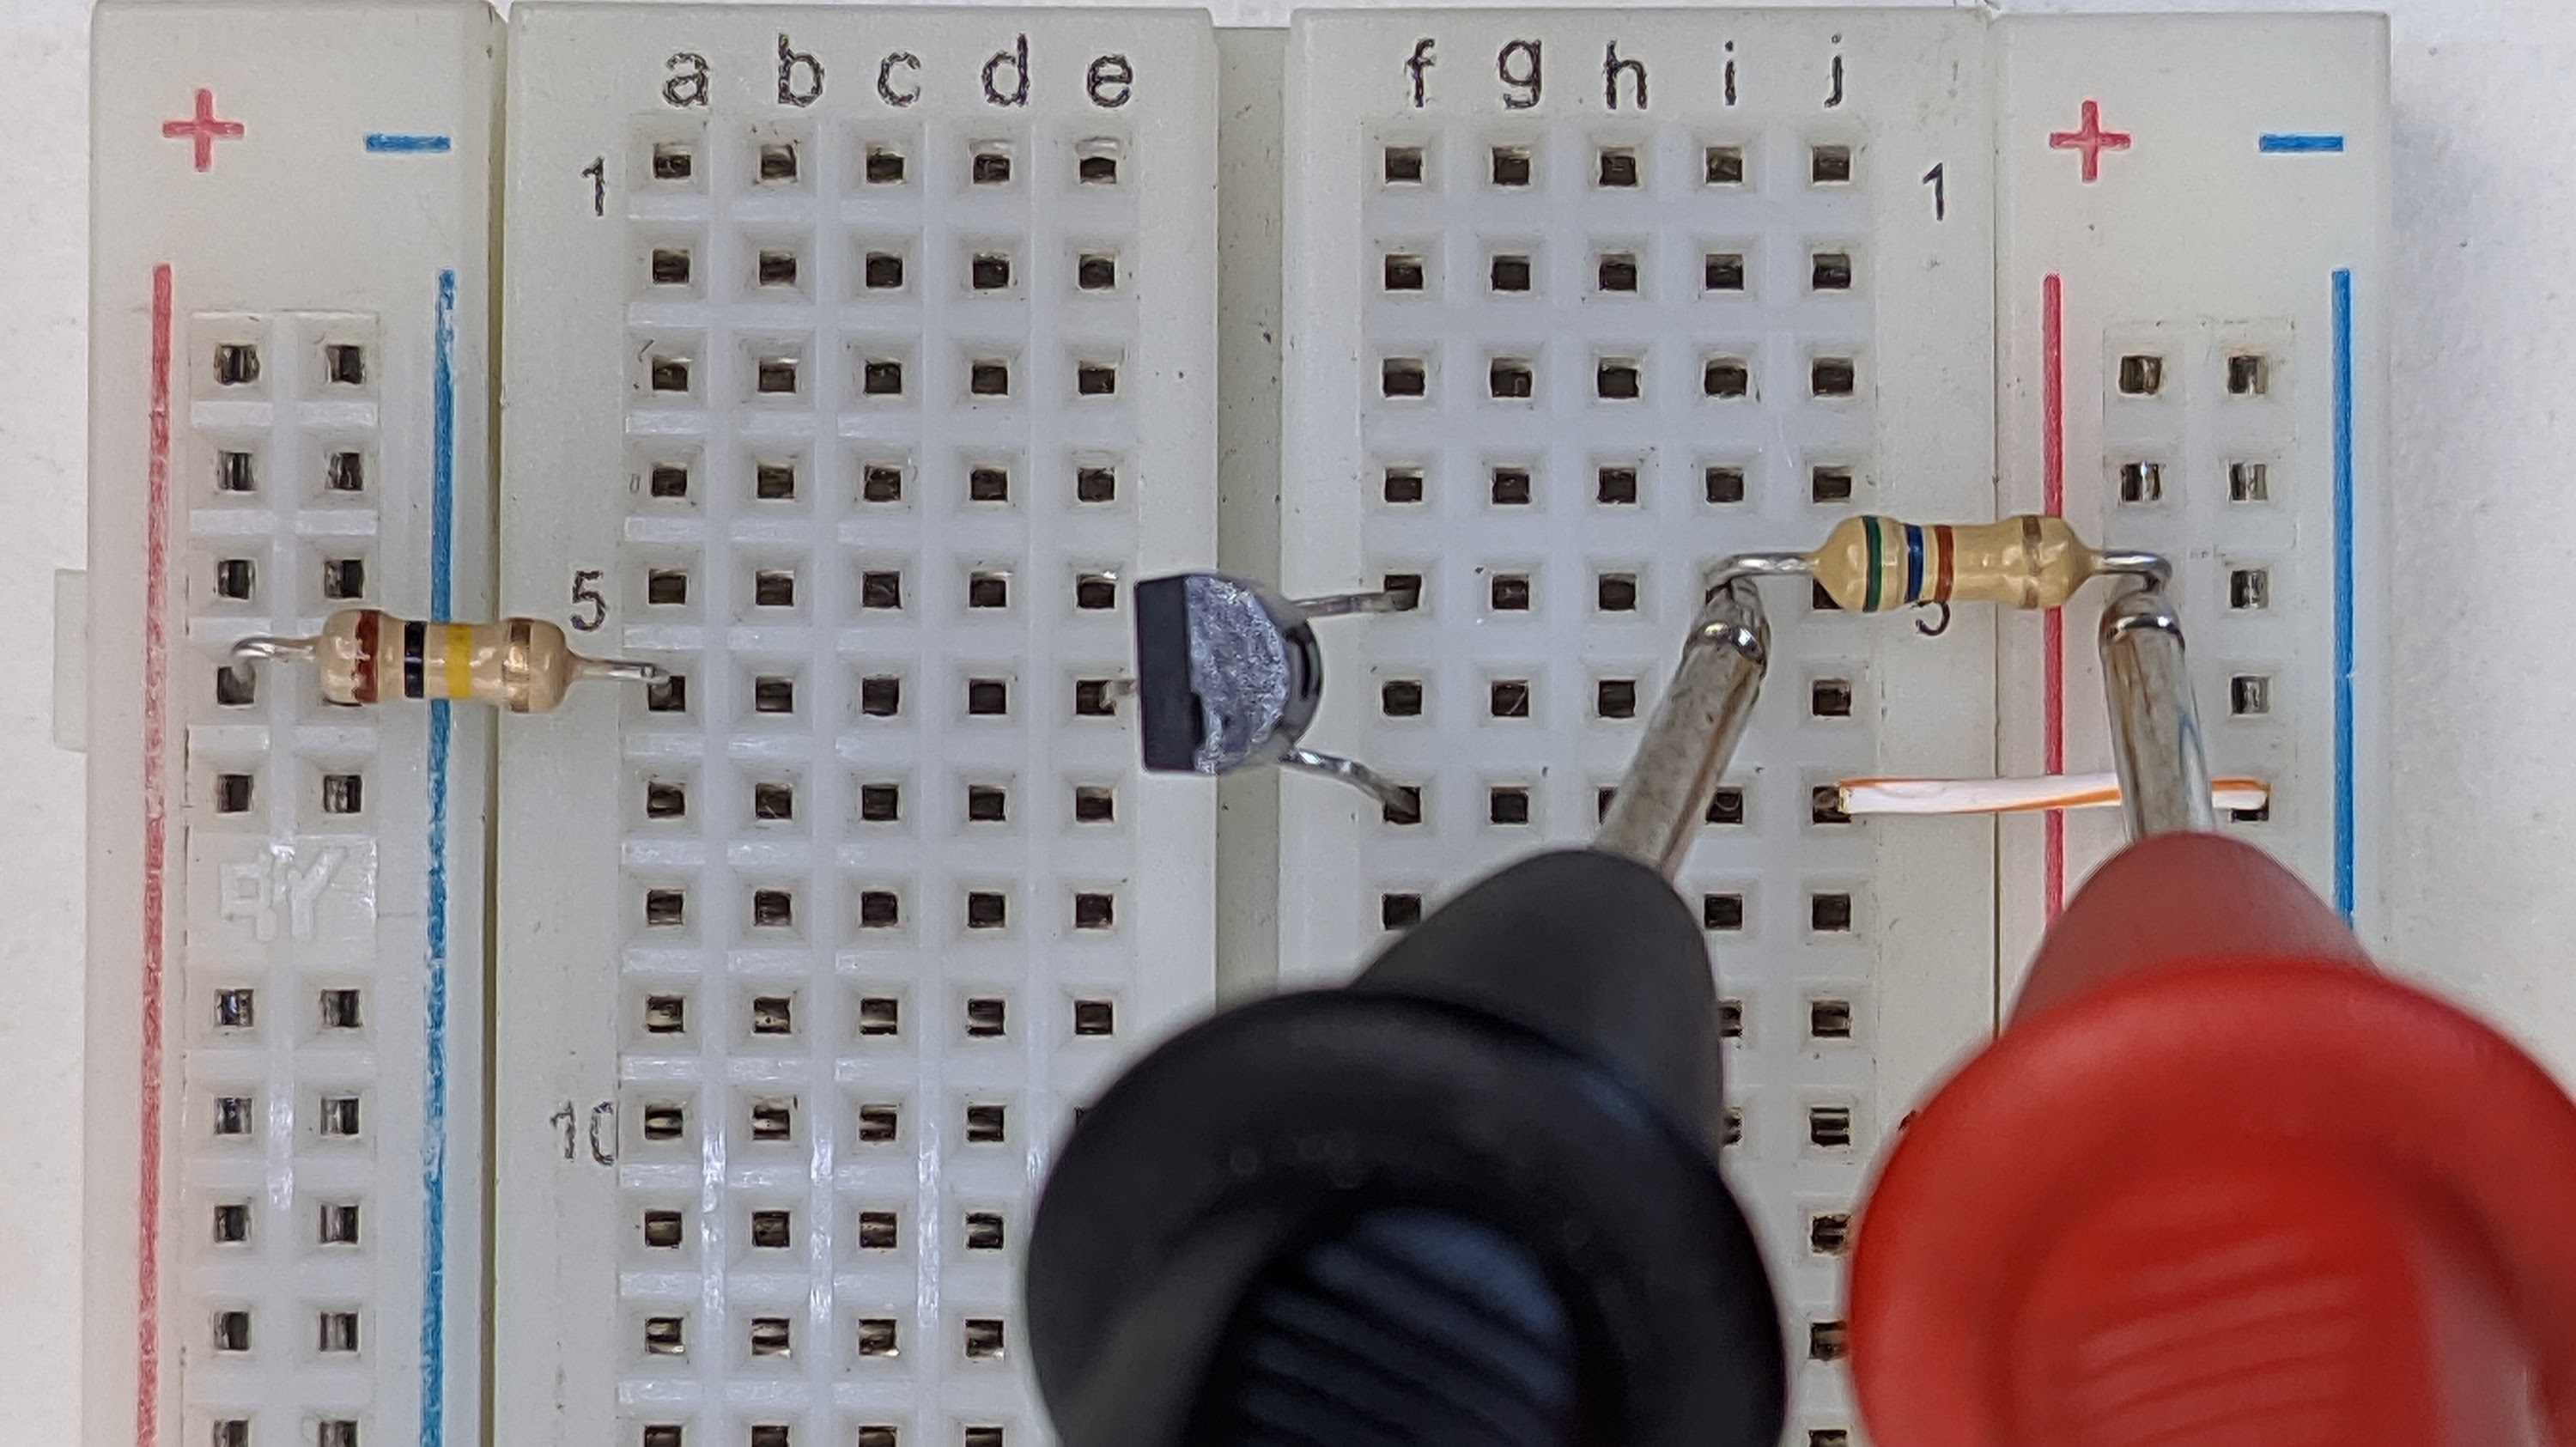
\includegraphics[width=1\textwidth]{pictures/prot_crkt-3_Vrc.jpg}
        \caption{Mediciones de $V_{R_C}$.}
      \end{minipage}
    \end{figure}

      Para este circuito, tambien decidimos medir la corriente del colector de manera indirecta, por lo que los valores
      de $I_C$ son calculados con esta ecuacion:
      \begin{equation}
        I_C = \frac{V_{R_C}}{R_C}
      \end{equation}

    \begin{table}
      \centering
      \resizebox{\textwidth}{!}{
        \begin{tabular}{*{11}{|c}|}
          \hline
          \multirow{2}{4em}{\centering $V_{CC}$} & \multicolumn{2}{c|}{$I_B = 0 \, A$} & \multicolumn{2}{c|}{$I_B = 10 \, \mu A$} & \multicolumn{2}{c|}{$I_B = 15 \, \mu A$} & \multicolumn{2}{c|}{$I_B = 20 \, \mu A$} & \multicolumn{2}{c|}{$I_B = 25 \, \mu A$}\\ \cline{2-11}
                      & $I_C$         & $V_{CE}$      & $I_C$           & $V_{CE}$      & $I_C$           & $V_{CE}$      & $I_C$           & $V_{CE}$      & $I_C$           & $V_{CE}$\\ \hline
          $0 \, V$    & $71 \, nA$    & $0 \, V$      & $12 \, \mu A$   & $0 \, V$      & $3 \, \mu A$    & $0 \, V$      & $8 \, \mu A$    & $0 \, V$      & $16 \, \mu A$   & $0 \, V$     \\ \hline
          $0.25 \, V$ & $160 \, nA$   & $0.257 \, V$  & $308 \, \mu A$  & $0.08 \, V$   & $335 \, \mu A$  & $0.069 \, V$  & $337 \, \mu A$  & $0.059 \, V$  & $337 \, \mu A$  & $0.054 \, V$ \\ \hline
          $0.5 \, V$  & $267 \, nA$   & $0.493 \, V$  & $698 \, \mu A$  & $0.108 \, V$  & $735 \, \mu A$  & $0.094 \, V$  & $723 \, \mu A$  & $0.083 \, V$  & $760 \, \mu A$  & $0.075 \, V$ \\ \hline
          $1 \, V$    & $267 \, nA$   & $1 \, V$      & $1.54 \, mA$    & $0.151 \, V$  & $1.5 \, mA$     & $0.122 \, V$  & $1.63 \, mA$    & $0.112 \, V$  & $1.68 \, mA$    & $0.150 \, V$ \\ \hline
          $2 \, V$    & $232 \, nA$   & $2 \, V$      & $3 \, mA$       & $0.273 \, V$  & $3.31 \, mA$    & $0.173 \, V$  & $3.4 \, mA$     & $0.151 \, V$  & $3.36 \, mA$    & $0.138 \, V$ \\ \hline
          $5 \, V$    & $517 \, nA$   & $5 \, V$      & $1.95 \, mA$    & $3.96 \, V$   & $2.56 \, mA$    & $3.56 \, V$   & $3.1 \, mA$     & $3.26 \, V$   & $7.85 \, mA$    & $0.553 \, V$ \\ \hline
          $10 \, V$   & $1 \, \mu A$  & $10 \, V$     & $1.69 \, mA$    & $9.14 \, V$   & $2.39 \, mA$    & $8.75 \, V$   & $3.3 \, mA$     & $8.19 \, V$   & $5.34 \, mA$    & $7.19 \, V$  \\ \hline
        \end{tabular}
      }
      \caption{Tabla de valores de $I_C$ y $V_{CE}$ segun $V_{CC}$.}
    \end{table}

    \begin{figure}[!ht]
      \centering
      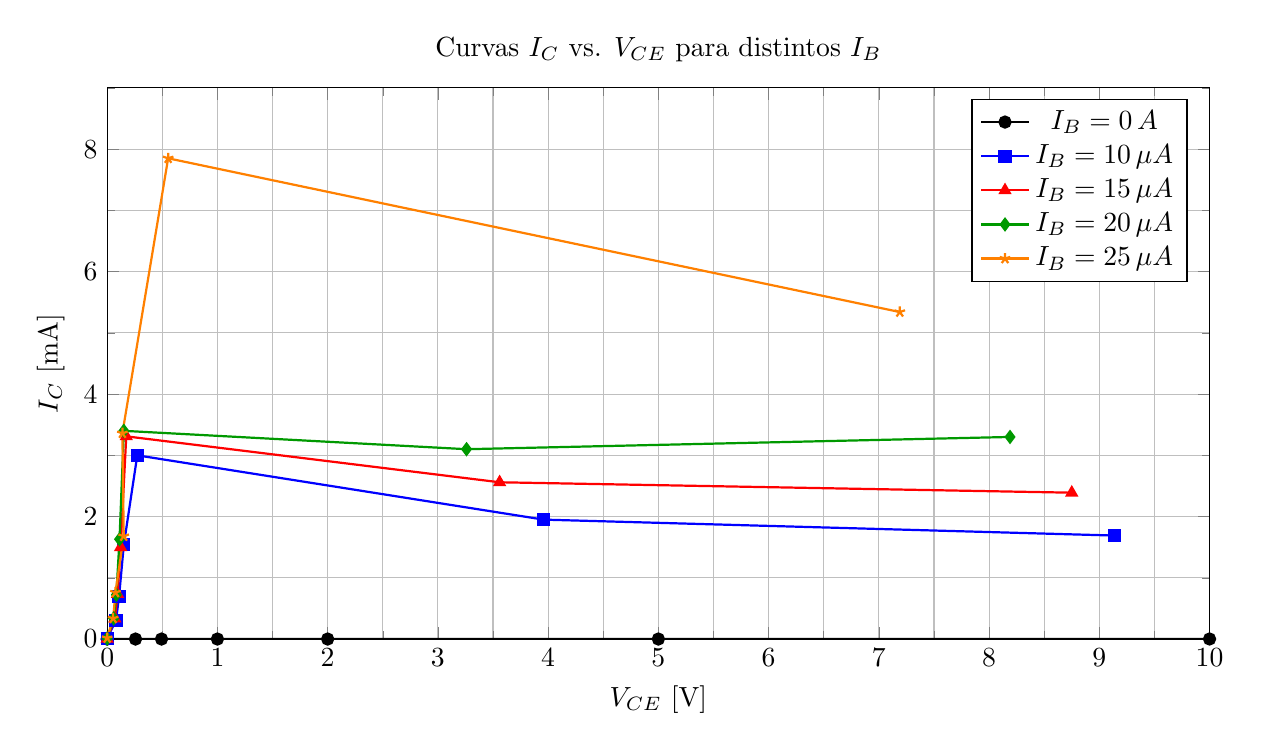
\begin{tikzpicture}
        \begin{axis}[
          width=14cm,
          height=7cm,
          xlabel={$V_{CE}$ [V]},
          ylabel={$I_C$ [mA]},
          grid=both,
          minor tick num=1,
          scale only axis,
          enlargelimits=false,
          title={Curvas $I_C$ vs. $V_{CE}$ para distintos $I_B$},
          scaled ticks=false,
          restrict x to domain=0:11,
          xmin=0, xmax=10,
          ymin=0, ymax=9
        ]

        % I_B = 0 A
        \addplot[
          mark=*,
          color=black,
          thick
        ] coordinates {
          (0, 0.000071)
          (0.257, 0.000160)
          (0.493, 0.000267)
          (1, 0.000267)
          (2, 0.000232)
          (5, 0.000517)
          (10, 0.001)
        };
        \addlegendentry{$I_B = 0 \, A$}

        % I_B = 10 uA
        \addplot[
          mark=square*,
          color=blue,
          thick
        ] coordinates {
          (0, 0.012)
          (0.08, 0.308)
          (0.108, 0.698)
          (0.151, 1.54)
          (0.273, 3)
          (3.96, 1.95)
          (9.14, 1.69)
        };
        \addlegendentry{$I_B = 10 \, \mu A$}

        % I_B = 15 uA
        \addplot[
          mark=triangle*,
          color=red,
          thick
        ] coordinates {
          (0, 0.003)
          (0.069, 0.335)
          (0.094, 0.735)
          (0.122, 1.5)
          (0.173, 3.31)
          (3.56, 2.56)
          (8.75, 2.39)
        };
        \addlegendentry{$I_B = 15 \, \mu A$}

        % I_B = 20 uA
        \addplot[
          mark=diamond*,
          color=green!60!black,
          thick
        ] coordinates {
          (0, 0.008)
          (0.059, 0.337)
          (0.083, 0.723)
          (0.112, 1.63)
          (0.151, 3.4)
          (3.26, 3.1)
          (8.19, 3.3)
        };
        \addlegendentry{$I_B = 20 \, \mu A$}

        % I_B = 25 uA
        \addplot[
          mark=star,
          color=orange,
          thick
        ] coordinates {
          (0, 0.016)
          (0.054, 0.337)
          (0.075, 0.760)
          (0.150, 1.68)
          (0.138, 3.36)
          (0.553, 7.85)
          (7.19, 5.34)
        };
        \addlegendentry{$I_B = 25 \, \mu A$}

        \end{axis}
      \end{tikzpicture}
    \end{figure}

    \begin{wrapfigure}{l}{0.4\textwidth}
      \centering
      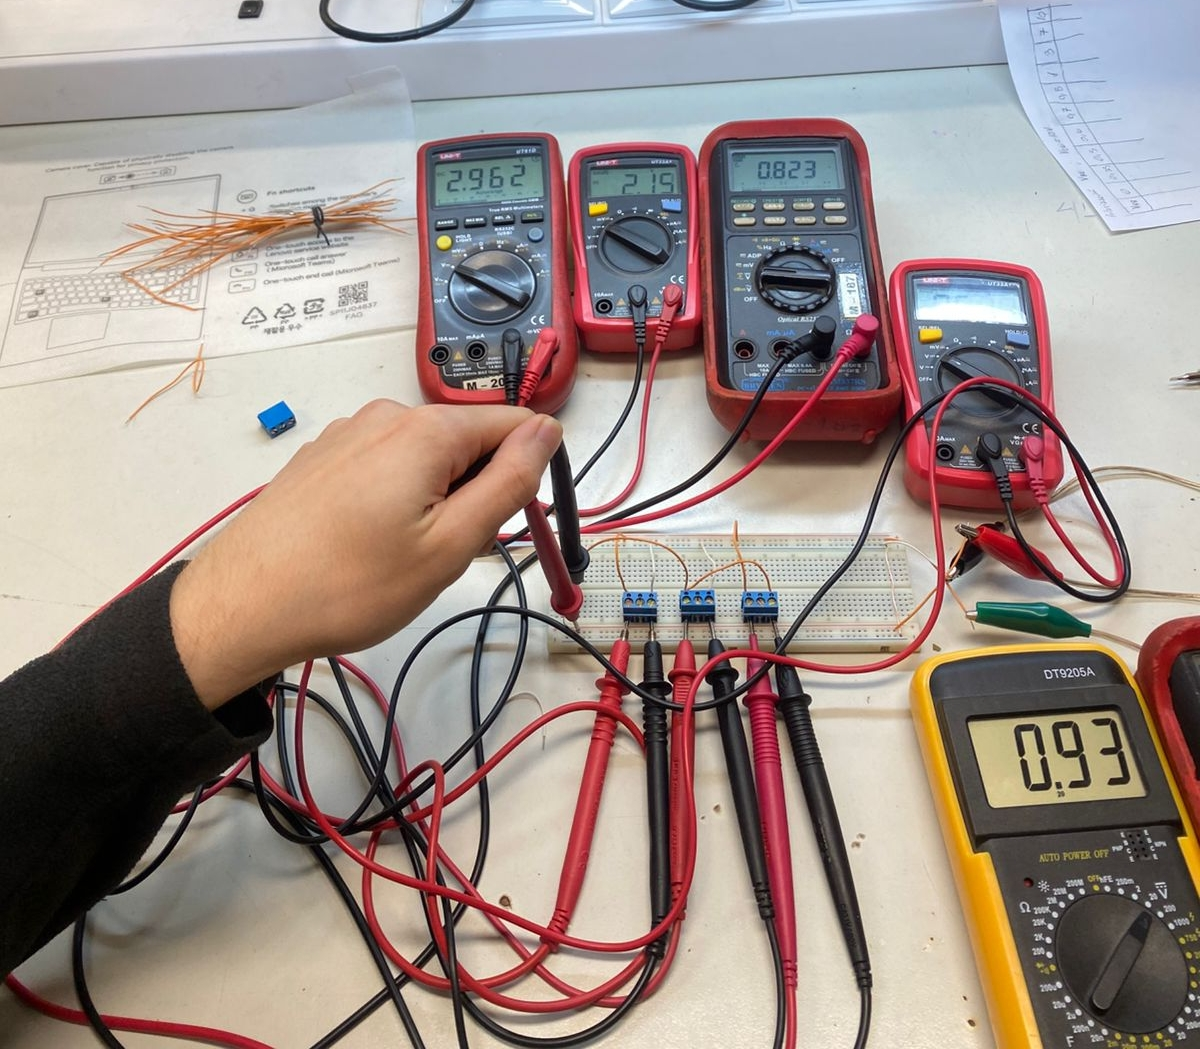
\includegraphics[width=0.35\textwidth]{pictures/setup_crkt-2.jpeg}
      \caption{Mediciones del circuito.}
    \end{wrapfigure}
    A partir del análisis experimental y simulado de las curvas características del transistor BJT, se identificaron
    claramente sus tres regiones de operación: corte, activa y saturación. Al mantener fija la corriente de base $I_B$ y
    barrer la tensión colector-emisor $V_{CE}$, se obtuvieron curvas $I_C$ vs.\ $V_{CE}$ que reflejan el comportamiento
    esperado del dispositivo.

    En la región activa se verificó una relación aproximadamente lineal entre $I_C$ e $I_B$, confirmando el modelo de
    amplificación controlada por corriente. En saturación, se observó que el transistor limita su capacidad de
    amplificación, mientras que en corte la corriente de colector fue prácticamente nula. La comparación entre los
    resultados de simulación y laboratorio mostró buena concordancia con la teoría, permitiendo validar el modelo del
    BJT como amplificador de señal o como conmutador, según el punto de operación elegido.
